\documentclass[10pt]{beamer}

\usetheme[progressbar=frametitle]{metropolis}
\usepackage{appendixnumberbeamer}

\usepackage{booktabs}
\usepackage[scale=2]{ccicons}
\usepackage{graphicx}
\graphicspath{ {./images/} }

\usepackage{pgfplots}
\usepackage{frcursive}
\usepackage{media9}
%\usepackage{multimedia}
\usepackage[T1]{fontenc}
\usepackage{hyperref}
\usepgfplotslibrary{dateplot}
\usepackage{xspace}
\usepackage{stmaryrd}
\usepackage{animate}
\usepackage{tcolorbox}

%%%%%%%%%%%%%%%%%%%%%%%%%%%%%%%%%%%%%%%%%%%%%%%%%%%%%%%%%%%%%%%%%%%%%%%%%%%%%%
% \embedvideo{<poster or text>}{<video file (MP4+H264)>}
%%%%%%%%%%%%%%%%%%%%%%%%%%%%%%%%%%%%%%%%%%%%%%%%%%%%%%%%%%%%%%%%%%%%%%%%%%%%%%
\usepackage[bigfiles]{pdfbase}
\ExplSyntaxOn
%%begin novalidate
\cs_new:Npn\embedvideo#1#2{
%%end novalidate
  \leavevmode
  \pbs_pdfobj:nnn{}{fstream}{{}{#2}}
  \pbs_pdfobj:nnn{}{dict}{
    /Type/Filespec/F~(#2)/UF~(#2)
    /EF~<</F~\pbs_pdflastobj:>>
  }
  \tl_set:Nx\video{\pbs_pdflastobj:}%
  %
  \pbs_pdfobj:nnn{}{dict}{
    /Type/RichMediaInstance/Subtype/Video
    /Asset~\video
    /Params~<</Binding/Foreground>>
  }
  %
  \pbs_pdfobj:nnn{}{dict}{
    /Type/RichMediaConfiguration/Subtype/Video
    /Instances~[\pbs_pdflastobj:]
  }
  %
  \pbs_pdfobj:nnn{}{dict}{
    /Type/RichMediaContent
    /Assets~<<
      /Names~[(#2)~\video]
    >>
    /Configurations~[\pbs_pdflastobj:]
  }
  \tl_set:Nx\rmcontent{\pbs_pdflastobj:}%
  %
  \pbs_pdfobj:nnn{}{dict}{
    /Activation~<<
      /Condition/XA
      /Presentation~<<
        /Transparent~true
        /Style/Embedded
        /PassContextClick~true
      >>
    >>
    /Deactivation~<</Condition/PC>>
  }
  %
  \hbox_set:Nn\l_tmpa_box{#1}
  \tl_set:Nx\l_box_wd_tl{\dim_use:N\box_wd:N\l_tmpa_box}
  \tl_set:Nx\l_box_ht_tl{\dim_use:N\box_ht:N\l_tmpa_box}
  \tl_set:Nx\l_box_dp_tl{\dim_use:N\box_dp:N\l_tmpa_box}
  \pbs_pdfxform:nnnnn{1}{1}{}{}{\l_tmpa_box}
  %
  \pbs_pdfannot:nnnn{\l_box_wd_tl}{\l_box_ht_tl}{\l_box_dp_tl}{
    /Subtype/RichMedia
    /BS~<</W~0/S/S>>
    /Contents~(embedded~video~file:#2)
    /NM~(rma:#2)
    /AP~<</N~\pbs_pdflastxform:>>
    /RichMediaSettings~\pbs_pdflastobj:
    /RichMediaContent~\rmcontent
  }
  \phantom{#1}
}%
\ExplSyntaxOff
%%%%%%%%%%%%%%%%%%%%%%%%%%%%%%%%%%%%%%%%%%%%%%%%%%%%%%%%%%%%%%%%%%%%%%%%%%%%%%


\newcommand{\themename}{\textbf{\textsc{metropolis}}\xspace}
\newcommand{\setfont}[2]{{\fontfamily{#1}\selectfont #2}}



\definecolor{lightgreen}{HTML}{EBF5E0}  % light green
\definecolor{greentheme}{HTML}{7eb356}  % green
\definecolor{orangetheme}{HTML}{ea9010}  % orange

\setbeamercolor{structure}{fg=greentheme, bg=orangetheme!40}
\setbeamercolor{alerted text}{fg=greentheme}
\setbeamercolor{progress bar}{greentheme}
\setbeamercolor{title separator}{greentheme}
\setbeamercolor{progress bar in head/foot}{greentheme}
\setbeamercolor{progress bar in section page}{greentheme}

\newcommand{\order}[1]{{\ensuremath{#1^{\mathrm{th}}}}}
\newcommand{\mat}[1]{\mathbf{#1}}
\newcommand{\femb}{h_{\mathrm{emb}}}
\newcommand{\fdet}{f_{\mathrm{det}}}
\newcommand{\fset}{\mathcal{F}}
\newcommand{\fdist}{\rho}
\newcommand{\perr}{P_{\mathrm{err}}}
\newcommand{\fext}{g_{\mathrm{ext}}}
\renewcommand{\vec}[1]{\mathbf{#1}}
\newcommand{\pcover}{P_{\mathcal{X}}}
\newcommand{\xcover}{{\mathcal{X}}}
\newcommand{\imspace}{{\mathcal{I}}}
\newcommand{\keys}{{\mathcal{K}}}
\newcommand{\msgs}{{\mathcal{M}}}
\newcommand{\xstegos}[1]{{\mathcal{Y}^{#1}}}
\newcommand{\zstegos}[1]{{\mathcal{Z}^{#1}}}
\newcommand{\pstego}{P_{\mathcal{Y}}}
\newcommand{\hfset}{\mathcal{F}}

\DeclareMathOperator*{\argmin}{arg\,min} % thin space, limits underneath in displays
\DeclareMathOperator*{\argmax}{arg\,max}

\title{Digital images steganography using adversarial embedding}
\subtitle{PhD's defense}
% \date{\today}
\date{18th October, 2021}
\author{Solène Bernard with Tom\'{a}\v{s} Pevn\'{y}, Patrick Bas and John Klein}
%\institute{IEEE Transactions on Information Forensics and Security, 2020}
% \titlegraphic{\hfill\includegraphics[height=1.5cm]{logo.pdf}}

\begin{document}

%\begin{frame}[standout]
\maketitle
%\end{frame}

\begin{frame}{Table of contents}
  \setbeamertemplate{section in toc}[sections numbered]
  \tableofcontents[hideallsubsections]
\end{frame}

\section{Introduction}


\begin{frame}{Context}
\begin{center}
\fbox{\begin{minipage}{24em}

\setfont{frc}{Dear Bob,

Would you like to listen my new interpretation of Satie? I just published it on Soundcloud. Please be honest. 

Cheers,

Alice
}
\end{minipage}}
\end{center}
\end{frame}



\begin{frame}{Context}
\begin{figure}[h]
    
\includegraphics[width=0.4\textwidth]{images/soundcloud_logo_2.png}\\\vspace{2em}
    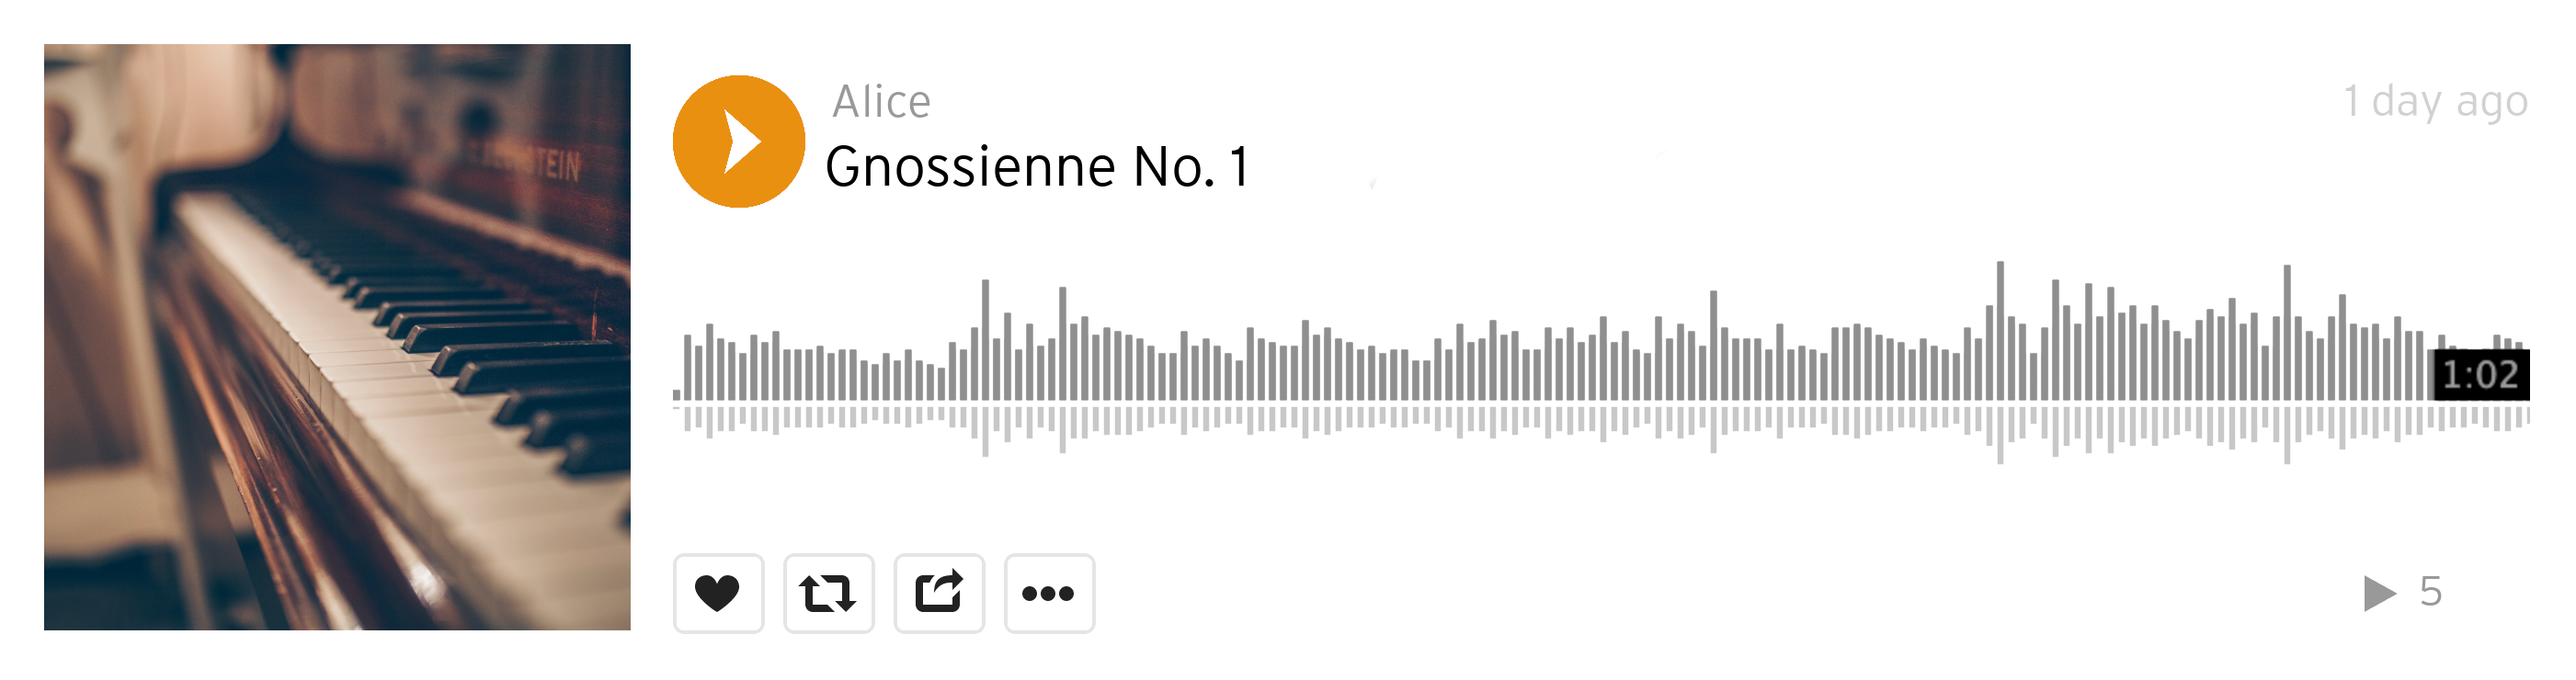
\includegraphics[width=\textwidth]{images/soundcloud.png}%
    \includemedia[addresource=stego.mp3,flashvars={source=stego.mp3,&autoPlay=false}]{Play}{APlayer.swf}
    %\href{run:stego.mp3}{\beamerbutton{Play}}
    %\sound{Play}{stego.mp3}
\end{figure}
\end{frame}


\begin{frame}{Context}
 \begin{figure}[h]
    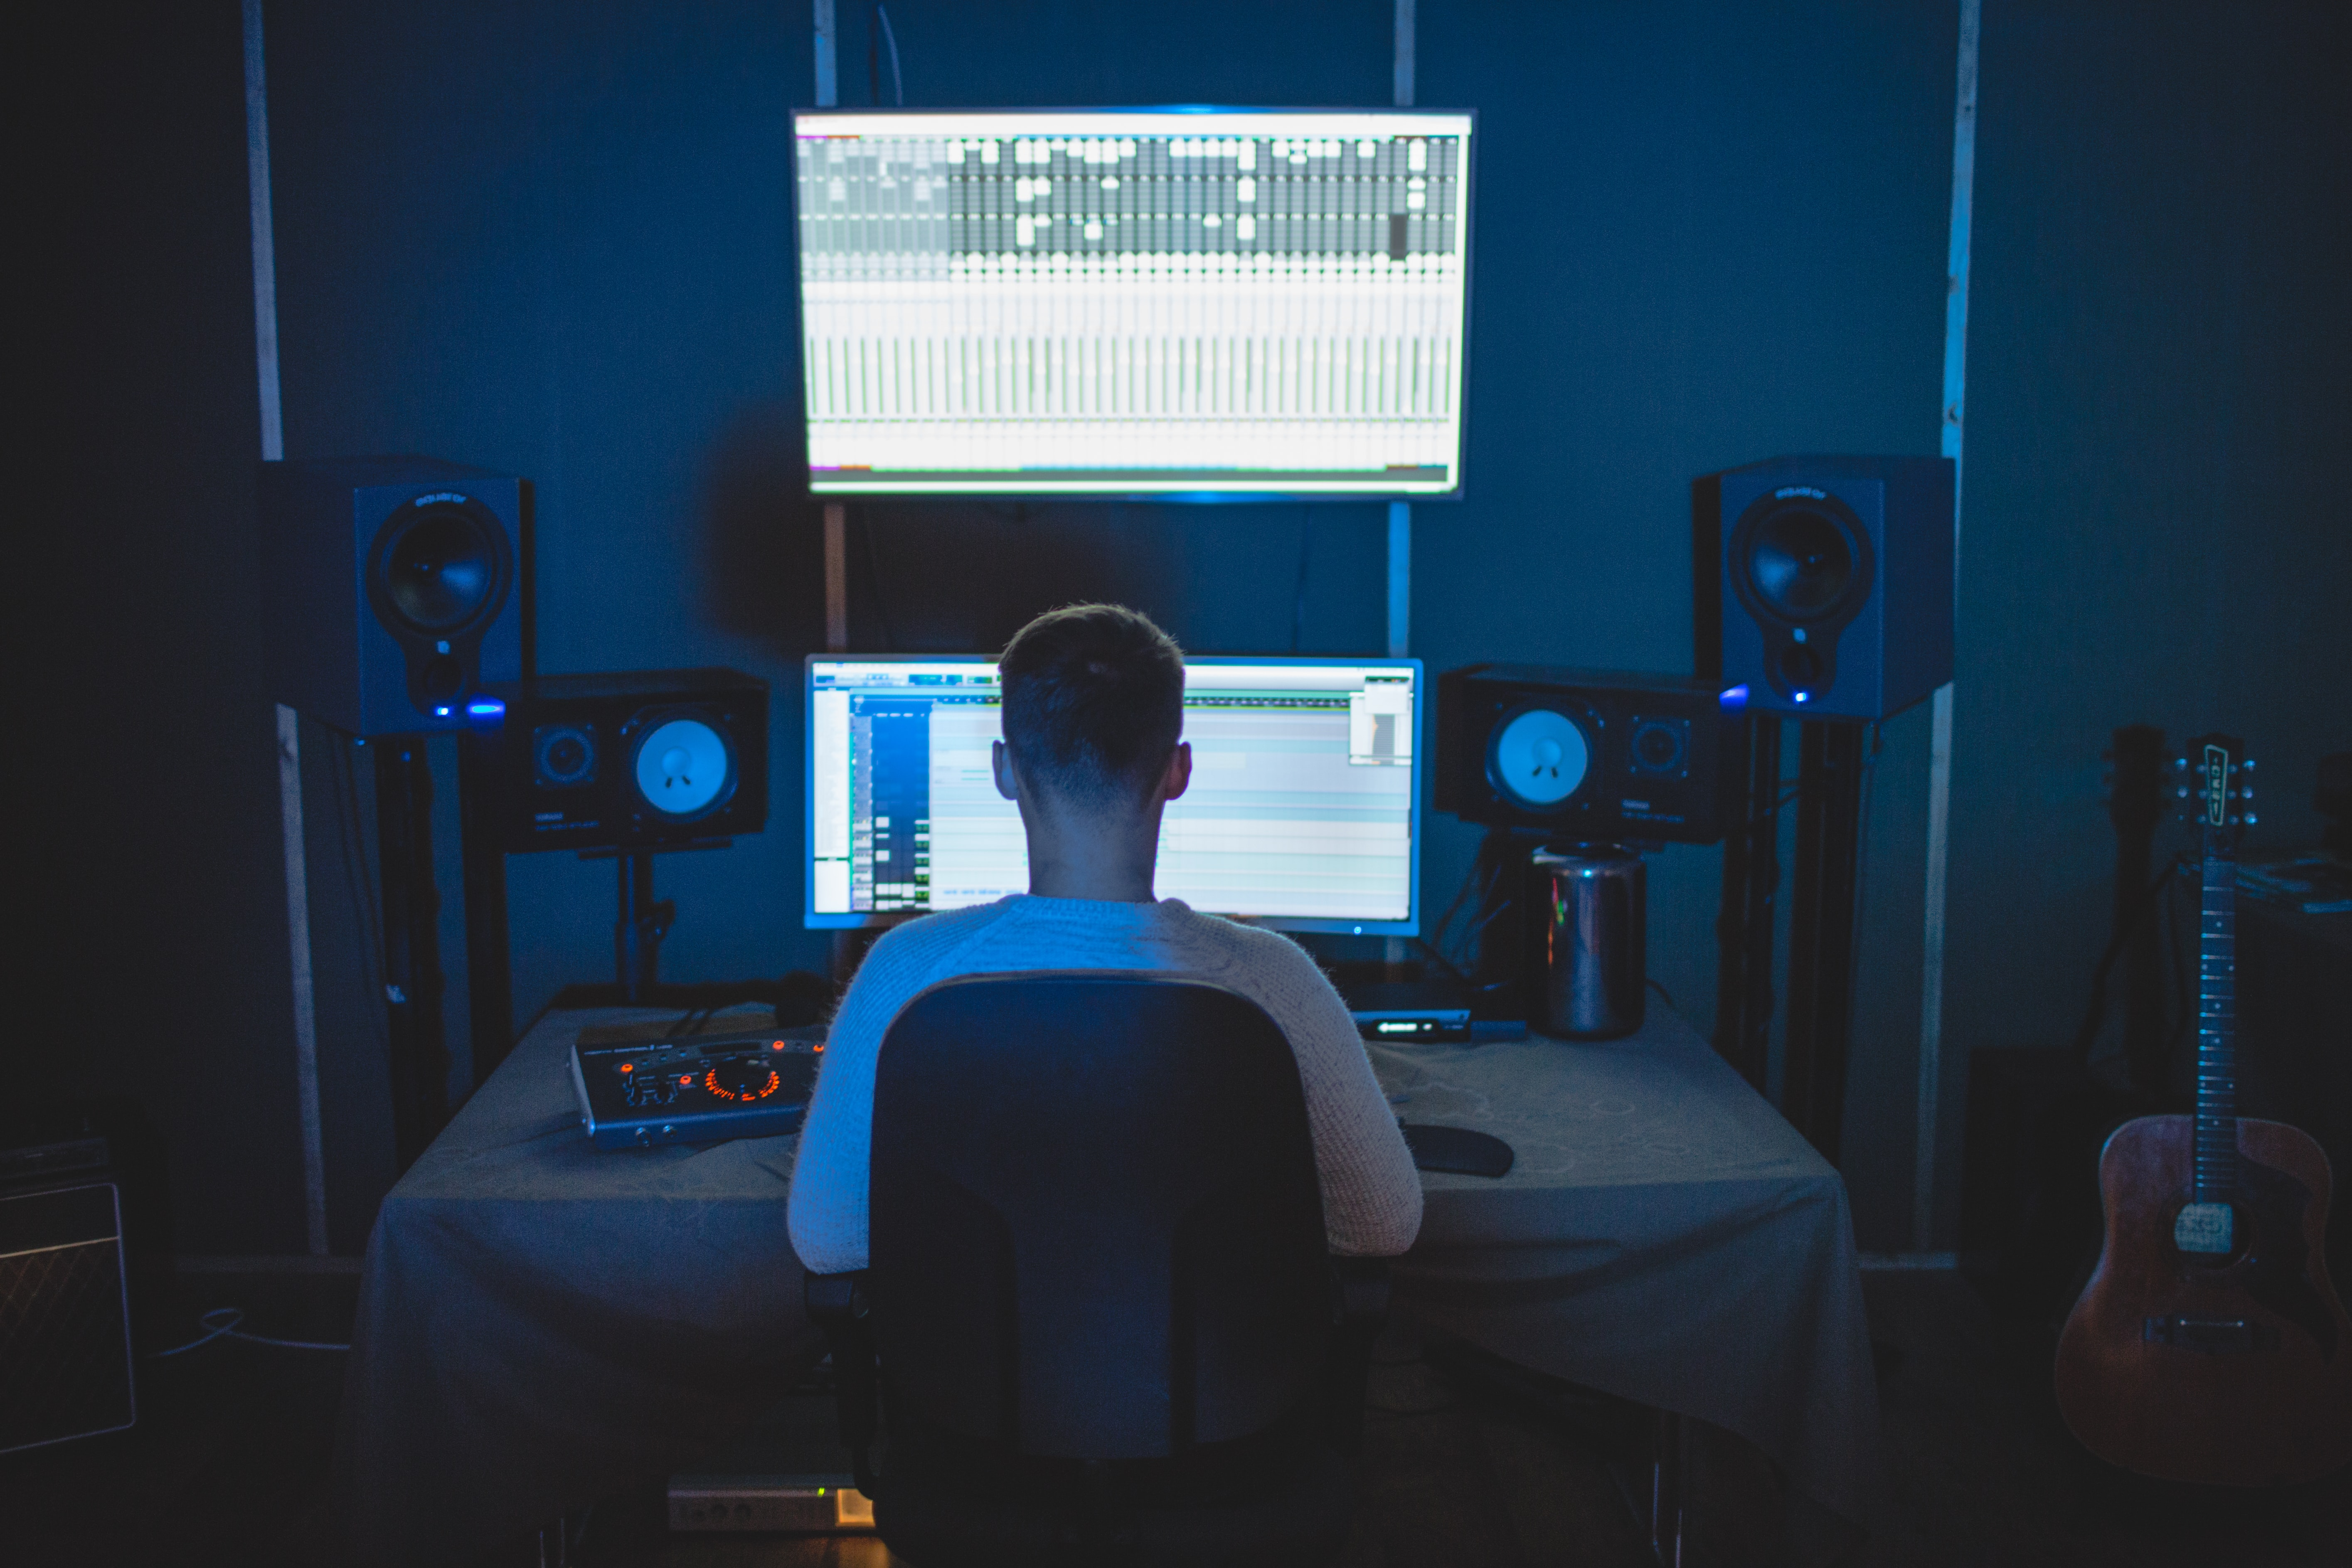
\includegraphics[width=0.9\textwidth]{images/computer.jpg}%
\end{figure}
\end{frame}


\begin{frame}{Context}
\animategraphics[width=\linewidth]{30}{animation_speed/image_}{0}{59}
\includemedia[addresource=stegodecode.mp3,flashvars={source=stegodecode.mp3,&autoPlay=false}]{Play}{APlayer.swf}
\end{frame}


\begin{frame}{Context}
\begin{figure}[h]
\includegraphics[width=\linewidth]{images/schema_stego3.pdf}
\end{figure}
\end{frame}

%\begin{frame}{Context}
%\alert{Kerckhoffs’s principle}

%Eve knows everything about Alice's strategy, except the secret key.

%"Worst-case scenario".
%\end{frame}

\section{Steganography with digital images}



\begin{frame}{Digital image structure}
Pixel values between 0 and 255. They are coded with 8 bits.
\begin{figure}[h]
\includegraphics[width=\linewidth]{images/image_structure.pdf}
\end{figure}
\end{frame}

\begin{frame}{LSB replacement}
Steganography by cover modification. Adding -1, 0 or +1 to pixels.

\alert{LSB} = "\alert{L}east \alert{S}ignificant \alert{B}it"
\begin{figure}[h]
\includegraphics[width=\linewidth]{images/lsbreplacement2.pdf}
\end{figure}
\end{frame}

\begin{frame}{LSB replacement}
\textit{Natural} images might have strong \alert{statistical features}.
\begin{figure}[h]
\includegraphics[width=\linewidth]{images/estonie_LSB.pdf}
\end{figure}
\end{frame}

\begin{frame}{LSB replacement}
\textit{Natural} images might have strong \alert{statistical features}.
\begin{figure}[h]
\includegraphics[width=\linewidth]{images/estonie_random.pdf}
%\caption{Gray scaled image, and display of the LSB of each pixel}
\end{figure}
\end{frame}

\begin{frame}{Cost of modification}
\begin{figure}[h]
\includegraphics[width=0.7\linewidth]{images/cost.pdf}
\end{figure}
\end{frame}

\begin{frame}{Cost of modification}
The detectability map is formed by the costs \alert{$\{\rho_i^b\}_i$} of changing the $i$-th pixel by adding value $b$.

In practice, the $\rho_i$ are usually computed from the cover image $\mathbf{x}$ using \alert{heuristic principles}.

Example:
\begin{itemize}
    \item In the JPEG domain:
        \begin{itemize}
            \item HUGO~\cite{hugo}
            \item J-UNIWARD~\cite{juni}
            \item SI-UNIWARD~\cite{juni}
            \item UERD~\cite{uerd}
        \end{itemize}
    \item In the spatial domain:
        \begin{itemize}
            \item HILL~\cite{hill}
        \end{itemize}
\end{itemize}

\end{frame}

\begin{frame}{Cost of modification}
\begin{figure}[h]
\includegraphics[width=\linewidth]{images/estoniecostmap.pdf}
\end{figure}
\end{frame}

\begin{frame}{Embedding a message}

\begin{tcolorbox}[colback=lightgreen,colframe=greentheme,title=\textbf{Definition} (The Payload-Limited Sender)]
The Payload-Limited Sender (PLS) attempts to find a distribution $\pi$ that communicates a required payload $|m|$ while minimizing the distortion $D(\mathbf{x},\mathbf{y}) = \sum_i \rho_i^{y_i - x_i}$:
\begin{equation}
\begin{array}{cc}
\operatorname{minimize} & \mathbb{E}_{\pi}[D]=\sum_{\mathbf{y} \in \mathcal{Y}(\mathbf{x})} \pi(\mathbf{y}) D(\mathbf{x}, \mathbf{y}) \\\\
 \mbox{ subject to } & H(\pi) = -\sum_{\mathbf{y} \in \mathcal{Y}(\mathbf{x})} \pi(\mathbf{y}) \log_{2} \pi(\mathbf{y}) =|m|
\end{array}
\end{equation}

\end{tcolorbox}

\end{frame}


\begin{frame}{Embedding a message}

\begin{tcolorbox}[colback=lightgreen,colframe=greentheme,title=\textbf{Theorem} (Optimal distribution w.r.t. distortion)]

For a given cover $\mathbf{x}$, an additive cost map $\{\rho_i^b\}_i$, and the set of reachable stegos $\mathcal{Y}(\mathbf{x})$, the solution of the PLS problem is reached for the following distribution:

\begin{equation}
\pi^{\star}(\mathbf{y})=\prod_{i}^{n} \frac{e^{-\lambda \rho_{i}^{y_{i}-x_{i}}}}{\sum_{b \in \mathbb{F}_{q}} e^{-\lambda \rho_{i}^{b}}}=\prod_{i}^{n} \pi_{i}^{\star}\left(y_{i}-x_{i}\right)
\end{equation}

with the following definition of the marginal probabilities:

\begin{equation}
\pi_{i}^{\star}(b)=\frac{e^{-\lambda \rho_{i}^{b}}}{\sum_{b^{\prime} \in \mathbb{F}_{q}} e^{-\lambda \rho_{i}^{b^{\prime}}}}
\end{equation}

where $\lambda$ is determined either from the entropy constraint:

\begin{equation}
H(\pi^{\star}) =|m|
\end{equation}

\end{tcolorbox}


\end{frame}

\begin{frame}{Simulated steganography}

Pipeline from the cover to the simulated stego:

\begin{equation*}
\begin{array}{ccccccccc}
    \mathbf{x} & \longrightarrow & \{\rho_i\}_i & \longrightarrow & \{\pi_i^b\}_i &   \xrightarrow{\mbox{\footnotesize{draw}}} & \{b_i\}_i &  \longrightarrow & \mathbf{y} = \mathbf{x} + \mathbf{b} \\ \\
    \mbox{\footnotesize{cover}} & & \mbox{\footnotesize{costs}} & & \mbox{\footnotesize{probabilities}} & & \mbox{\footnotesize{changes}} & &  \mbox{\footnotesize{stego}}
    
\end{array}
\end{equation*}
\end{frame}


\begin{frame}{Simulated steganography}
\begin{figure}[h]
\includegraphics[width=\linewidth]{images/estoniepmap.pdf}
%\caption{Heuristic cost of modification $\rho_i = \rho_i^{-1} = \rho_i^{+1}$ (given by HILL algorithm).}
\end{figure}
\end{frame}

%\begin{frame}{Detectability map}
%The embedding operation (named HUGO, J-UNIWARD,S-UNIWARD, ...) can be simulated by changing each pixel $i$ by probability $p_i$ given by : 
%\begin{equation}
%    p_i = \frac{\exp(-\lambda \rho_i)}{1+\exp(-\lambda \rho_i)}
%\end{equation}
%where $\lambda>0$ is a constant determined by the constraint of the size of the message $m$ :
%\begin{equation}
%    m = \sum_{i=1}^{i=n} H(p_i)
%\end{equation}
%\end{frame}

%\begin{frame}{Probability map}
%    \begin{figure}[h]
%        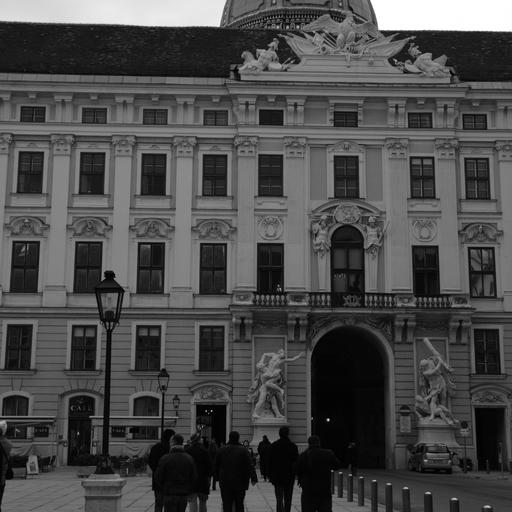
\includegraphics[scale=0.3]{13}
%        \caption{Image from BOSS base}
%    \end{figure}
%\end{frame}
    
%\begin{frame}{Probability map}
%    \begin{figure}[h]
%        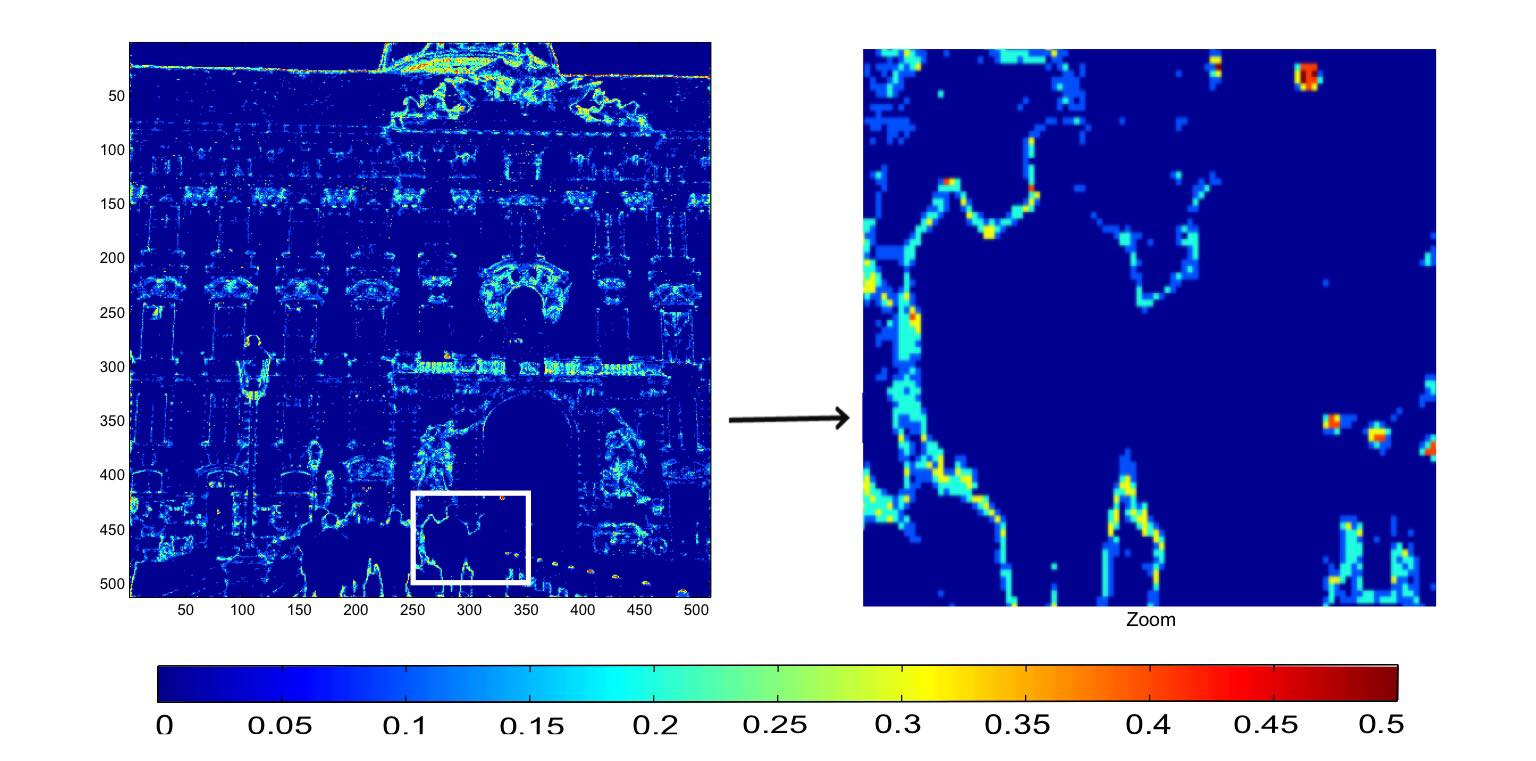
\includegraphics[scale=0.2]{probabilities}
%        \caption{Probability map of embedding for the same image when HUGO steganographic scheme is used at 0.2 bpp}
%    \end{figure}
%\end{frame}


\section{Steganalysis}


\begin{frame}{Steganalysis}
Steganalysis is Eve's role. It is the antagonist art of steganography. 

\alert{The purpose is to detect the presence of a hidden message in an image.}

\end{frame}

\begin{frame}{Deep learning}
\animategraphics[width=\linewidth]{30}{animation_training/}{0}{50}
\end{frame}


\begin{frame}{Deep learning for steganalysis}
\animategraphics[width=\linewidth]{30}{animation_training_stega/}{0}{50}
\end{frame}


\begin{frame}{Steganalysis}

Classifier to discriminate between cover and stego images. 


\pause
For example XU-Net~\cite{xu2017deep}, SRNet~\cite{boroumand2018deep}.

Notation: $f : \mathcal{I} \rightarrow [0,1]$.
\begin{equation*}
    \left\{
    \begin{array}{ll}
    f(\mathbf{x}) < 0.5 & \mbox{ if } \mathbf{x}\mbox{ cover} \\
    f(\mathbf{x}) \geq 0.5 & \mbox{ if } \mathbf{x}\mbox{ stego} \\
    \end{array}
    \right.
\end{equation*}
\end{frame}


\begin{frame}{Adversarial steganography}

Pingpong, cat-and-mouse game.
Automatic game
Loop between Alice and Eve
Connection with Andrew and MiPod

Adversarial example: ADV-EMB
\minmax
    
\end{frame}

\section{Playing an iterative game with a $\min\max$ protocol}


\begin{frame}{The $\min\max$ protocol}
\alert{Approximating Alice's objective by an iterative $\minmax$ strategy.} 

\pause
Initialization: $\mathcal{A}_e = \fset^{0} = \{f^0\}$,  $\mathcal{A}_a = \{\mathcal{Z}^0\}$.
\pause

At~$k^{\mathrm{th}}$ iteration, the two following macro-steps: 
\begin{enumerate}
	\item \alert<2>{Alice's turn.} 
	\begin{equation}
	\mathbf{z}^\ast = \arg \min_{\mathbf{z} \in \mathcal{A}_a} \max_{f \in \fset^{k-1}} f(\mathbf{z});
	\label{eq:stepone}	
	\end{equation}
    \pause
	\item \alert<3>{Eve's turn.} Creation of a new detector $\fdet^k$ and appends it to the pool, i.e. $\fset^k = \fset^{k-1} \cup \{\fdet^k\}.$
\end{enumerate}
\end{frame}



\begin{frame}{Past contribution}
  \begin{figure}
        \includegraphics[width=\linewidth]{images/increasing_game_0.pdf}
\end{figure}
\end{frame}

\begin{frame}{Past contribution}
  \begin{figure}
        \includegraphics[width=\linewidth]{images/increasing_game_1.pdf}
\end{figure}
\end{frame}


\begin{frame}{Past contribution}
  \begin{figure}
        \includegraphics[width=\linewidth]{images/increasing_game_1_bis.pdf}
\end{figure}
\end{frame}


\begin{frame}{Past contribution}
  \begin{figure}
        \includegraphics[width=\linewidth]{images/increasing_game_2.pdf}
\end{figure}
\end{frame}

\begin{frame}{Past contribution}
  \begin{figure}
        \includegraphics[width=\linewidth]{images/increasing_game_2_bis.pdf}
\end{figure}
\end{frame}

\begin{frame}{Past contribution}
  \begin{figure}
        \includegraphics[width=\linewidth]{images/increasing_game_3.pdf}
\end{figure}
\end{frame}


\begin{frame}{Past contribution}
  \begin{figure}
        \includegraphics[width=\linewidth]{images/increasing_game_4.pdf}
\end{figure}
\end{frame}


\begin{frame}{Past contribution}
  \begin{figure}
        \includegraphics[width=\linewidth]{images/increasing_game_5.pdf}
\end{figure}
\end{frame}



\begin{frame}{Goal: optimizing the cost map}

\begin{equation*}
    \begin{array}{ll}
    \mathbf{x} \longrightarrow \rho_i \longrightarrow p_i \alert<3>{\xrightarrow{-1, +0, +1}} \mathbf{y} \longrightarrow \max f(\mathbf{y})
    \\ \pause
    \hspace{3em} \alert{\xleftarrow{\hspace{5em} \nabla_\rho f(\mathbf{y}) \hspace{3em}}} \pause
    \end{array}
\end{equation*}

\end{frame}


\begin{frame}{Practical solution: optimizing the cost map with ADV-EMB}

%Goal: optimize $\rho$ w.r.t. $f(\mathbf{y})$.  \pause So we want to compute \alert<2>{\nabla_{\mathbf{\rho}}f(\mathbf{y})}. 

%\pause
%\begin{equation*}
%     \mathbf{x} \longrightarrow \rho_i \longrightarrow p_i \alert<3>{ \xrightarrow{-1, +0, +1}} \mathbf{y} \longrightarrow f(\mathbf{y})
% \end{equation*}
% \pause
ADV-EMB~\footfullcite{tang2019cnn}: heuristic method to update \alert<1>{costs} of modifications given the sign of the gradient of a classifier.
\pause
\begin{equation*}
    \begin{array}{cc}
    \mathbf{x} \hspace{2.2em} \alert<3>{\rho_i} \hspace{2.2em} p_i \hspace{4.4em} \mathbf{y} \alert<2-3-4>{\xleftarrow{\text{sign }\nabla_{\mathbf{y}}f}} f(\mathbf{y}) \\ \pause
    \hspace{2em} \alert<3>{\xdashleftarrow{\text{\hspace{5em} heuristic \hspace{5em}}}}
    \end{array}
\end{equation*}
\pause
\begin{equation}
\rho_{i}^{+, new} = 
\left\{
    \begin{array}{ll}
        \rho_{i}^+/\alpha & \mbox{if } \alert<4>{\frac{\partial f}{\partial y_{i}}\left(\mathbf{y}\right)} < 0, \\
        \rho_{i}^+ & \mbox{if } \alert<4>{\frac{\partial f}{\partial y_{i}}\left(\mathbf{y}\right)} = 0, \\
        \rho_{i}^+ \alpha & \mbox{if } \alert<4>{\frac{\partial f}{\partial y_{i}}\left(\mathbf{y}\right)} > 0,
    \end{array}
\right.
\label{eq:qplus}
\end{equation}
\pause
\begin{equation}
\arg \min_{\mathbf{z} \in \mathcal{A}_a} f(\mathbf{z}), \quad  f \in \fset^{k-1}
\end{equation}
\pause
Then $\min\max$ strategy to compute $\mathbf{z}^\ast$.

\end{frame}



\begin{frame}{Results}
Multiple figures
\end{frame}


\begin{frame}{Flaws of ADV-EMB}
    \begin{figure}
        \includegraphics[width=\linewidth]{images/minmax_evolution_it1.pdf}
    \end{figure}
\end{frame}


\begin{frame}{Flaws of ADV-EMB}
    \begin{figure}
        \includegraphics[width=\linewidth]{images/minmax_evolution_it2.pdf}
    \end{figure}
\end{frame}


\begin{frame}{Flaws of ADV-EMB}
    \begin{figure}
        \includegraphics[width=\linewidth]{images/minmax_evolution_it3.pdf}
    \end{figure}
\end{frame}

\begin{frame}{Flaws of ADV-EMB}
    \begin{figure}
        \includegraphics[width=\linewidth]{images/minmax_evolution_it4.pdf}
    \end{figure}
\end{frame}

\begin{frame}{Flaws of ADV-EMB}
    \begin{figure}
        \includegraphics[width=\linewidth]{images/minmax_evolution_it5.pdf}
    \end{figure}
\end{frame}

\begin{frame}{Flaws of ADV-EMB}
    \begin{figure}
        \includegraphics[width=\linewidth]{images/minmax_evolution_it6.pdf}
    \end{figure}
\end{frame}

\begin{frame}{Flaws of ADV-EMB}
    \begin{figure}
        \includegraphics[width=\linewidth]{images/minmax_evolution_it7.pdf}
    \end{figure}
\end{frame}

\begin{frame}{Flaws of ADV-EMB}
    \begin{figure}
        \includegraphics[width=\linewidth]{images/minmax_evolution_it8.pdf}
    \end{figure}
\end{frame}

\begin{frame}{Flaws of ADV-EMB}
    \begin{figure}
        \includegraphics[width=\linewidth]{images/minmax_evolution_it9.pdf}
    \end{figure}
%\pause
% \begin{itemize}
%     \item New stegos defeats only the last classifier \pause
%     \item The $\min \max$ value reaches too quickly the ceil value.
% \end{itemize}
\end{frame}


\begin{frame}{Flaws of ADV-EMB}
    \begin{itemize}
      
        
        \item At some point, it fails at solving  
        \begin{equation*}
            \mathbf{z}^\ast = \arg \min_{\mathbf{z} \in \mathcal{A}_a} \max_{f \in \fset^{k-1}} f(\femb(\mathbf{x}));
        \end{equation*} 
        
        \pause
          \item Heuristic
    \end{itemize}
\end{frame}


\section{Second contribution: Backpack}


\begin{frame}{Backpack}
\alert{Backpack}: \alert{Back-p}ropagable att\alert{ack} \pause in order to compute \alert{$\nabla_{\rho} f(\mathbf{y})$}.

    \begin{equation*}
        \begin{array}{ll}
        \mathbf{x} \longrightarrow \rho_i \longrightarrow p_i \xrightarrow{-1, +0, +1} \mathbf{y} \longrightarrow f(\mathbf{y})
        \\ \pause
        \hspace{3em} \alert{\xleftarrow{\hspace{5em} \nabla_\rho f(\mathbf{y}) \hspace{3em}}}
        \end{array}
    \end{equation*}
    
    \pause
   \begin{enumerate}
       \item Approximation of discrete modification by continuous modifications controlled by a temperature $\tau$ 
       \begin{equation*}
       \begin{array}{ll}
            \mathbf{x} \longrightarrow \rho_i \longrightarrow p_i \alert{ \xrightarrow{\tilde{b}_\tau}} \tilde{\mathbf{y}} \longrightarrow f(\tilde{\mathbf{y}}) %\\ \pause
        %\hspace{6em} \alert{\xleftarrow{\hspace{0em} \nabla_p \tilde{\mathbf{y}_i} \hspace{0em}}} 
        \end{array}
        \end{equation*}
    
        \pause
       \item Computation of the gradient thanks to the gradient of a function defined implicitly
         \begin{equation*}
         \begin{array}{ll}
            \mathbf{x} \longrightarrow \rho_i \alert{\longrightarrow} p_i  \xrightarrow{\tilde{b}_\tau} \tilde{\mathbf{y}} \longrightarrow f(\tilde{\mathbf{y}}) %\\ \pause
        %\hspace{3em} \alert{\xleftarrow{\hspace{0em} \nabla_\rho p_i \hspace{0em}}} 
        \end{array}
        \end{equation*}
   \end{enumerate}
\end{frame}


% \begin{frame}{1. Approximation of discrete modifications}
%     \pause 
%     How to draw from the following categorical distribution? 
%     \begin{table}[h]
%         \centering
%         \begin{tabular}{c||c|c|c}
%             b & -1  & 0 & 1   \\ \hline
%             p & p^{-1}  & p^0 & p^{+1}   \\
%         \end{tabular} 
%         \hspace{2em} with $p^{-1} + p^0 + p^{+1} = 1$
%         \label{tab:probalaw}
%     \end{table}
    
%     % Two solutions:
%     % \begin{table}[h]
%     %     \centering
%     %     \begin{tabular}{c|c}
%     %         $u \sim U(0,1)$ & $g^{-1},g^{0},g^{+1}  \sim G(0,1)$ \\
%     %         $b =\left\{
%     %             \begin{array}{ll}
%     %               -1 & \text{ if } u < p^{-1}\\
%     %               0 & \text{ elif } u < p^{-1}+p^0\\ 
%     %               +1 & \text{ else}
%     %             \end{array}
%     %           \right.$
             
%     %          & $b = \argmax_{j \in\{-1,0,1\}} g^{j} + \log p^j$
%     %     \end{tabular}
%     %   \label{tab:drawlaw}
%     % \end{table}
%     \pause
%     Possible solution: draw $g^{-1},g^{0},g^{+1}  \sim G(0,1)$, then
%     \begin{equation}
%         b = \argmax_{j \in\{-1,0,1\}} g^{j} + \log p^j
%     \end{equation}  \pause
    
%     \begin{equation}
%         \mbox{one-hot}\left(\argmax_{j \in\{-1,0,1\}} g^{j} + \log p^j\right) = \alert{\lim_{\tau \rightarrow 0} \softmax_{j \in\{-1,0,1\}}\left(\frac{g^{j} + \log p^j}{\tau}\right)}
%     \end{equation}

% \end{frame}

\begin{frame}{1. Approximation of discrete modifications with Softmax Gumbel distribution}
    \begin{figure}[h]
        \includegraphics[width=\linewidth]{images/ternarychanges_softmaxgumbel.pdf}
    \end{figure}
\end{frame}



\begin{frame}{2. $\frac{\partial \mathbf{p}}{\partial \rho}$ computed implicitly}

    Probabilities are a function of costs $\rho$ and $\lambda$
    \begin{equation}
        p_i^j = P_i^j\left(\rho_{i}, \lambda\right)%=\frac{e^{-\lambda \rho_{i}^{j}}}{\sum_{k \in \mathcal{B}} e^{-\lambda \rho_{i}^{k}}}, \quad j \in \{-1, 0, 1\}
    \end{equation}
    
    \pause
    
    but $\lambda = \alert{\Lambda(\rho,|\mathbf{m}|))}$ is an (implicit) function of $\rho$ and $|m|$ stemming from the entropy constraint:
    
    \begin{equation}
        H\left(\left(p_i^j\right)_{i,j}\right)=|\mathbf{m}|
    \end{equation}
    
    \pause
    
    Explicit gradient of $\lambda$ accessible through differentiation of the entropy constraint.
    
\end{frame}



% \begin{frame}{2. $\frac{\partial \mathbf{p}}{\partial \rho}$ computed implicitly}

%     Full expression of the gradient :
%     \begin{equation}
%         \frac{\partial \mathbf{p}}{\partial \rho}=\frac{\partial P_{\mathbf{b}}}{\partial \rho} \frac{\partial \rho}{\partial \rho}+\frac{\partial P_{\mathbf{b}}}{\partial \lambda} \alert{\frac{\partial \Lambda(\rho,|\mathbf{m}|))}{\partial \rho}}
%     \end{equation} \pause
%     But because the condition on entropy:
    
%     \begin{equation}
%         H\left(P_{\mathbf{b}}(\lambda, \rho)\right)=H\left(P_{\mathbf{b}}(\Lambda(\rho,|\mathbf{m}|), \rho)\right)=|\mathbf{m}|
%     \end{equation} \pause
    
%     The derivative w.r.t. $\rho$ is equals to zero:
%     \begin{equation}
%         \frac{\partial H\left(P_{\mathbf{b}}\right)}{\partial \rho} \frac{\partial \rho}{\partial \rho}+\frac{\partial H\left(P_{\mathrm{b}}\right)}{\partial \lambda} \alert{\frac{\partial \Lambda}{\partial \rho}}=0
%     \end{equation}
% \end{frame}


\begin{frame}{Overall algorithm}


\alert{Backpack}: \alert{Back-p}ropagable att\alert{ack}.
   \begin{align*}
    \mathbf{x} \longrightarrow \rho_i \alert{\longrightarrow} p_i \alert{ \xrightarrow{\tilde{b}_\tau}} \tilde{\mathbf{y}} & \longrightarrow f(\tilde{\mathbf{y}}) %\\
    % & \longrightarrow f^1(\tilde{\mathbf{y}}) \\
    % & \dots \\
    % & \longrightarrow f^{k-1}(\tilde{\mathbf{y}})
    \end{align*}
\pause

Iterative gradient descent, while playing with the temperature $\tau$, to optimize the smooth output w.r.t. best detector:

\begin{equation}
    \alert{\nabla_{\rho} f(\tilde{\mathbf{y}})}, \quad  f = \argmax_{f \in \mathcal{F}^{k-1}} f(\tilde{\mathbf{y}})
\end{equation}

\end{frame}

\begin{frame}{Difference between smooth and discrete stegos}
    \begin{figure}[h]
        \includegraphics[width=\linewidth]{images/gradient_descent_purpose_tau.pdf}
    \end{figure}
\end{frame}


% \begin{frame}{Overall algorithm: hyperparameters}
% Hyperparameters:
%     \begin{itemize}
%         \item \alert<1>{Learning rate and optimizer} $\quad \alpha=5e^{-2}$ or $\alpha=5e^{-1}$ with ADAM. \pause
%         \item \alert<2>{Starting temperature $\tau_0$. }  $ \quad  \tau_0 = 1$. \pause
%         \item \alert<3>{When to decrease the temperature.} $\quad \max_f |f(\tilde{\mathbf{y}}) - f(\mathbf{x})| < \epsilon$. \pause
%         \item \alert<4>{How to decrease the temperature.} $\quad  \tau \leftarrow \tau/2$ \pause
%         \item \alert<5>{Stopping condition.} $\quad \max_f |f(\mathbf{y}) - f(\mathbf{x})| < \epsilon$. \pause
%         \item \alert<6>{Maximum number of steps.} 
%     \end{itemize}
% \end{frame}





\begin{frame}{Evolution of $\min\max$}
    \begin{figure}
        \includegraphics[width=\linewidth]{images/minmax_SGE_evolution_it1.pdf}
    \end{figure}
\end{frame}


\begin{frame}{Evolution of $\min\max$}
    \begin{figure}
        \includegraphics[width=\linewidth]{images/minmax_SGE_evolution_it2.pdf}
    \end{figure}
\end{frame}


\begin{frame}{Evolution of $\min\max$}
    \begin{figure}
        \includegraphics[width=\linewidth]{images/minmax_SGE_evolution_it3.pdf}
    \end{figure}
\end{frame}


\begin{frame}{Evolution of $\min\max$}
    \begin{figure}
        \includegraphics[width=\linewidth]{images/minmax_SGE_evolution_it4.pdf}
    \end{figure}
\end{frame}


\begin{frame}{Evolution of $\min\max$}
    \begin{figure}
        \includegraphics[width=\linewidth]{images/minmax_SGE_evolution_it5.pdf}
    \end{figure}
\end{frame}


\begin{frame}{Evolution of $\min\max$}
    \begin{figure}
        \includegraphics[width=\linewidth]{images/minmax_SGE_evolution_it6.pdf}
    \end{figure}
\end{frame}


\begin{frame}{Evolution of $\min\max$}
    \begin{figure}
        \includegraphics[width=\linewidth]{images/minmax_SGE_evolution_it7.pdf}
    \end{figure}
\end{frame}


\begin{frame}{Results}
    \begin{figure}
        \includegraphics[width=\linewidth]{images/results0.pdf}
    \end{figure}
\end{frame}


\begin{frame}{Results}
    \begin{figure}
        \includegraphics[width=\linewidth]{images/results1.pdf}
    \end{figure}
\end{frame}

\begin{frame}{Results}
    \begin{figure}
        \includegraphics[width=\linewidth]{images/results2.pdf}
    \end{figure}
\end{frame}

\begin{frame}{Results}
    \begin{figure}
        \includegraphics[width=\linewidth]{images/results3.pdf}
    \end{figure}
\end{frame}

\begin{frame}{Results}
eSRNet, eXuNet, correlations, comparison between eXUNet and XUNet at QF 100 ! ("very last updates")
"One more thing"X

    \begin{figure}[h]
        \includegraphics[width=0.75\linewidth]{images/QF75_3models.pdf}
    \end{figure}
    \pause
    \begin{center}
        \begin{tabular}{ccccc}
           \textbf{EfNet} & \textbf{XU-Net} & \textbf{SRNet} & DCTR & GFR \\
           \alert{$+31.6 \%$} & \alert{$+31.0\%$} & \alert{$+38.2 \%$} & $+20.5\%$ & $+27.0 \%$
        \end{tabular}
    \end{center}
    
\end{frame}


\section{Conclusion and perspectives}

\begin{frame}{Frame Title}
    Réfléchir !! S'inspirer des faiblesses. 
    Problems:
    \begin{itemize}
        \item Sooooo costly
        \item Transferability: source dependance, domain adaptation, self-supervised learning

    \end{itemize}

\end{frame}



\begin{frame}{Conclusion}
    Automatically improved steganography w.r.t. steganalysis. 
    \begin{figure}[h]
        \includegraphics[width=0.6\linewidth]{images/evedefeated.pdf}
    \end{figure}
\end{frame}


\bibliographystyle{acm}
\bibliography{demo}

\end{document}
